\section{Putting it together: PageRank}
\label{sec:pagerank}


The PageRank algorithm is the cornerstone of Google's search technology\cite{pagerank}. It is used to rank the many trillions of URLs by importance. PageRank iteratively updates a rank for each webpage by adding up contributions from each page that links to it. 

PageRank is an example of a difficult to parallelize in-memory computation. Part of the complexity arises from the complex pattern of data sharing which is often encountered in many graph algorithms \cite{pagerank}. The computation of the PageRank score of a web page is derived from the score of the ``neighboring'' web pages. The most bandwidth-hungry stage during a MapReduce implementation of PageRank is the iterative reduce step that aggregates the parent URL for a URL key to compute its rank. 

\subsection{PageRank with MapReduce on Meteor}

The PageRank algorithm can easily be described using the MapReduce programming model. The input to each of the MapReduce job is a \code{(url, (outlink_list, rank))} RDD. Each pair is passed in as input to the mapper which produces a set of all outlinked pages as keys with contribution as values. Contribution is computed from taking the rank of the origin page, divided by the total number of outlinks from the origin page. The reducer then updates each page rank by computing a weigted sum of the contributions each page received from the mapper stage. The PageRank algorithm is implemented in Spark using Resilient Distributed Datasets (RDDs) \cite{rdd} as follows:

%
\begin{lstlisting}[label=mapreduce] 

// Load graph as an RDD of (URL, outlinks) pairs
val links = spark.textFile(...).map(...).persist()
var ranks = // RDD of (URL, rank) pairs
for (i <- 1 to ITERATIONS) {
    // Build an RDD of (targetURL, float) pairs
    // with the contributions sent by each page
    val contribs = links.join(ranks).flatMap {
        (url, (links, rank)) =>
        links.map(dest => (dest, rank/links.size))
    }
    // Sum contributions by URL and get new ranks
    ranks = contribs.reduceByKey((x,y) => x+y)
        .mapValues(sum => a/N + (1-a)*sum)
}

\end{lstlisting}
%

We show the RDD lineage graph and the RDD stage dependencies for the PageRank job stages in Figure \ref{fig:lineage}. Each dotted box is an RDD and partitions are shown as shaded rectangles. Consider the simple example where we would like to compute PageRanks on datasets that are distributed across two nodes. While the goal of Meteor is to minimize communication between geographically distant data-centers, we suggest for the sake of simplicity to use the term 'node' loosely when covering the PageRank example.

\begin{figure}[!ht]
    \centering
    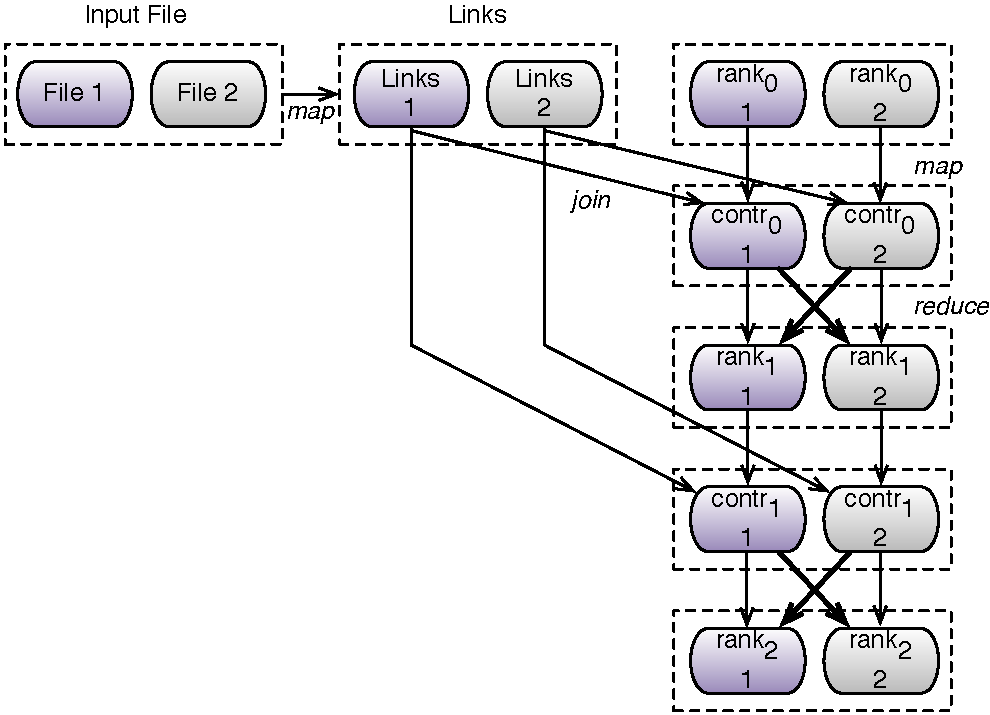
\includegraphics[width=\textwidth]{figs/lineage.pdf}
    \caption{Lineage and dependency graph for datasets in PageRank. Each dotted box is an RDD and partitions are shown as shaded rectangles.}
    \label{fig:lineage}
\end{figure}

The first stage of the PageRank algorithm is to load the input files, and parse them to generate a set of links from which the ranks of each page can get computed. Ideally, when loading the files, we would like the scheduler to choose an assignment that minimizes inter-node transfer while keeping the partitions balanced among the nodes. 

We address this first issue in Meteor by allowing the application to specify locality awareness and implement bandwidth aware work-stealing for improved load balancing, as discussed in section \ref{sec: design}. This ensures that loading the file data into RDDs generates as low as possible inter-node communication. Once the input files have been loaded into ``locality-aware'' partitions, the links datasets can be generated locally without requiring any inter-node communication. 

The iterative stages of PageRank rely on inter-node communication during the reduce phase in order to update the ranks of the pages which inlinks sit in a distant partition. In Spark, communication can be reduced by controlling how the RDDs get partitionned. By using \emph{consistent partitioning} across each iteration of the algorithm, specifically on the \code{links} and \code{ranks} sets, the \code{join} operation requires no inter-node communication. On top of consistent \emph{partitioning}, Spark permits the use of combiners \cite{hop} in order to minimize inter-node traffic by aggregating values by keys on the map side. 

Beyond consistent partitionining and combining, Meteor avoids inter-node traffic during the reduce stage by dropping updates performed at each MapReduce iteration. This technique effectively isolates the iterative PageRank computation on each partition until there is bandwidth available to update PageRanks across nodes. We present the benefits of this technique over Spark's execution in Section 4.

%\lstinputlisting[language=Java]{listings/PageRankPregel.java}

